\section{Scientific Domain Applications}
\label{sec:domain_applications}

\begin{figure*}[t]
\centering
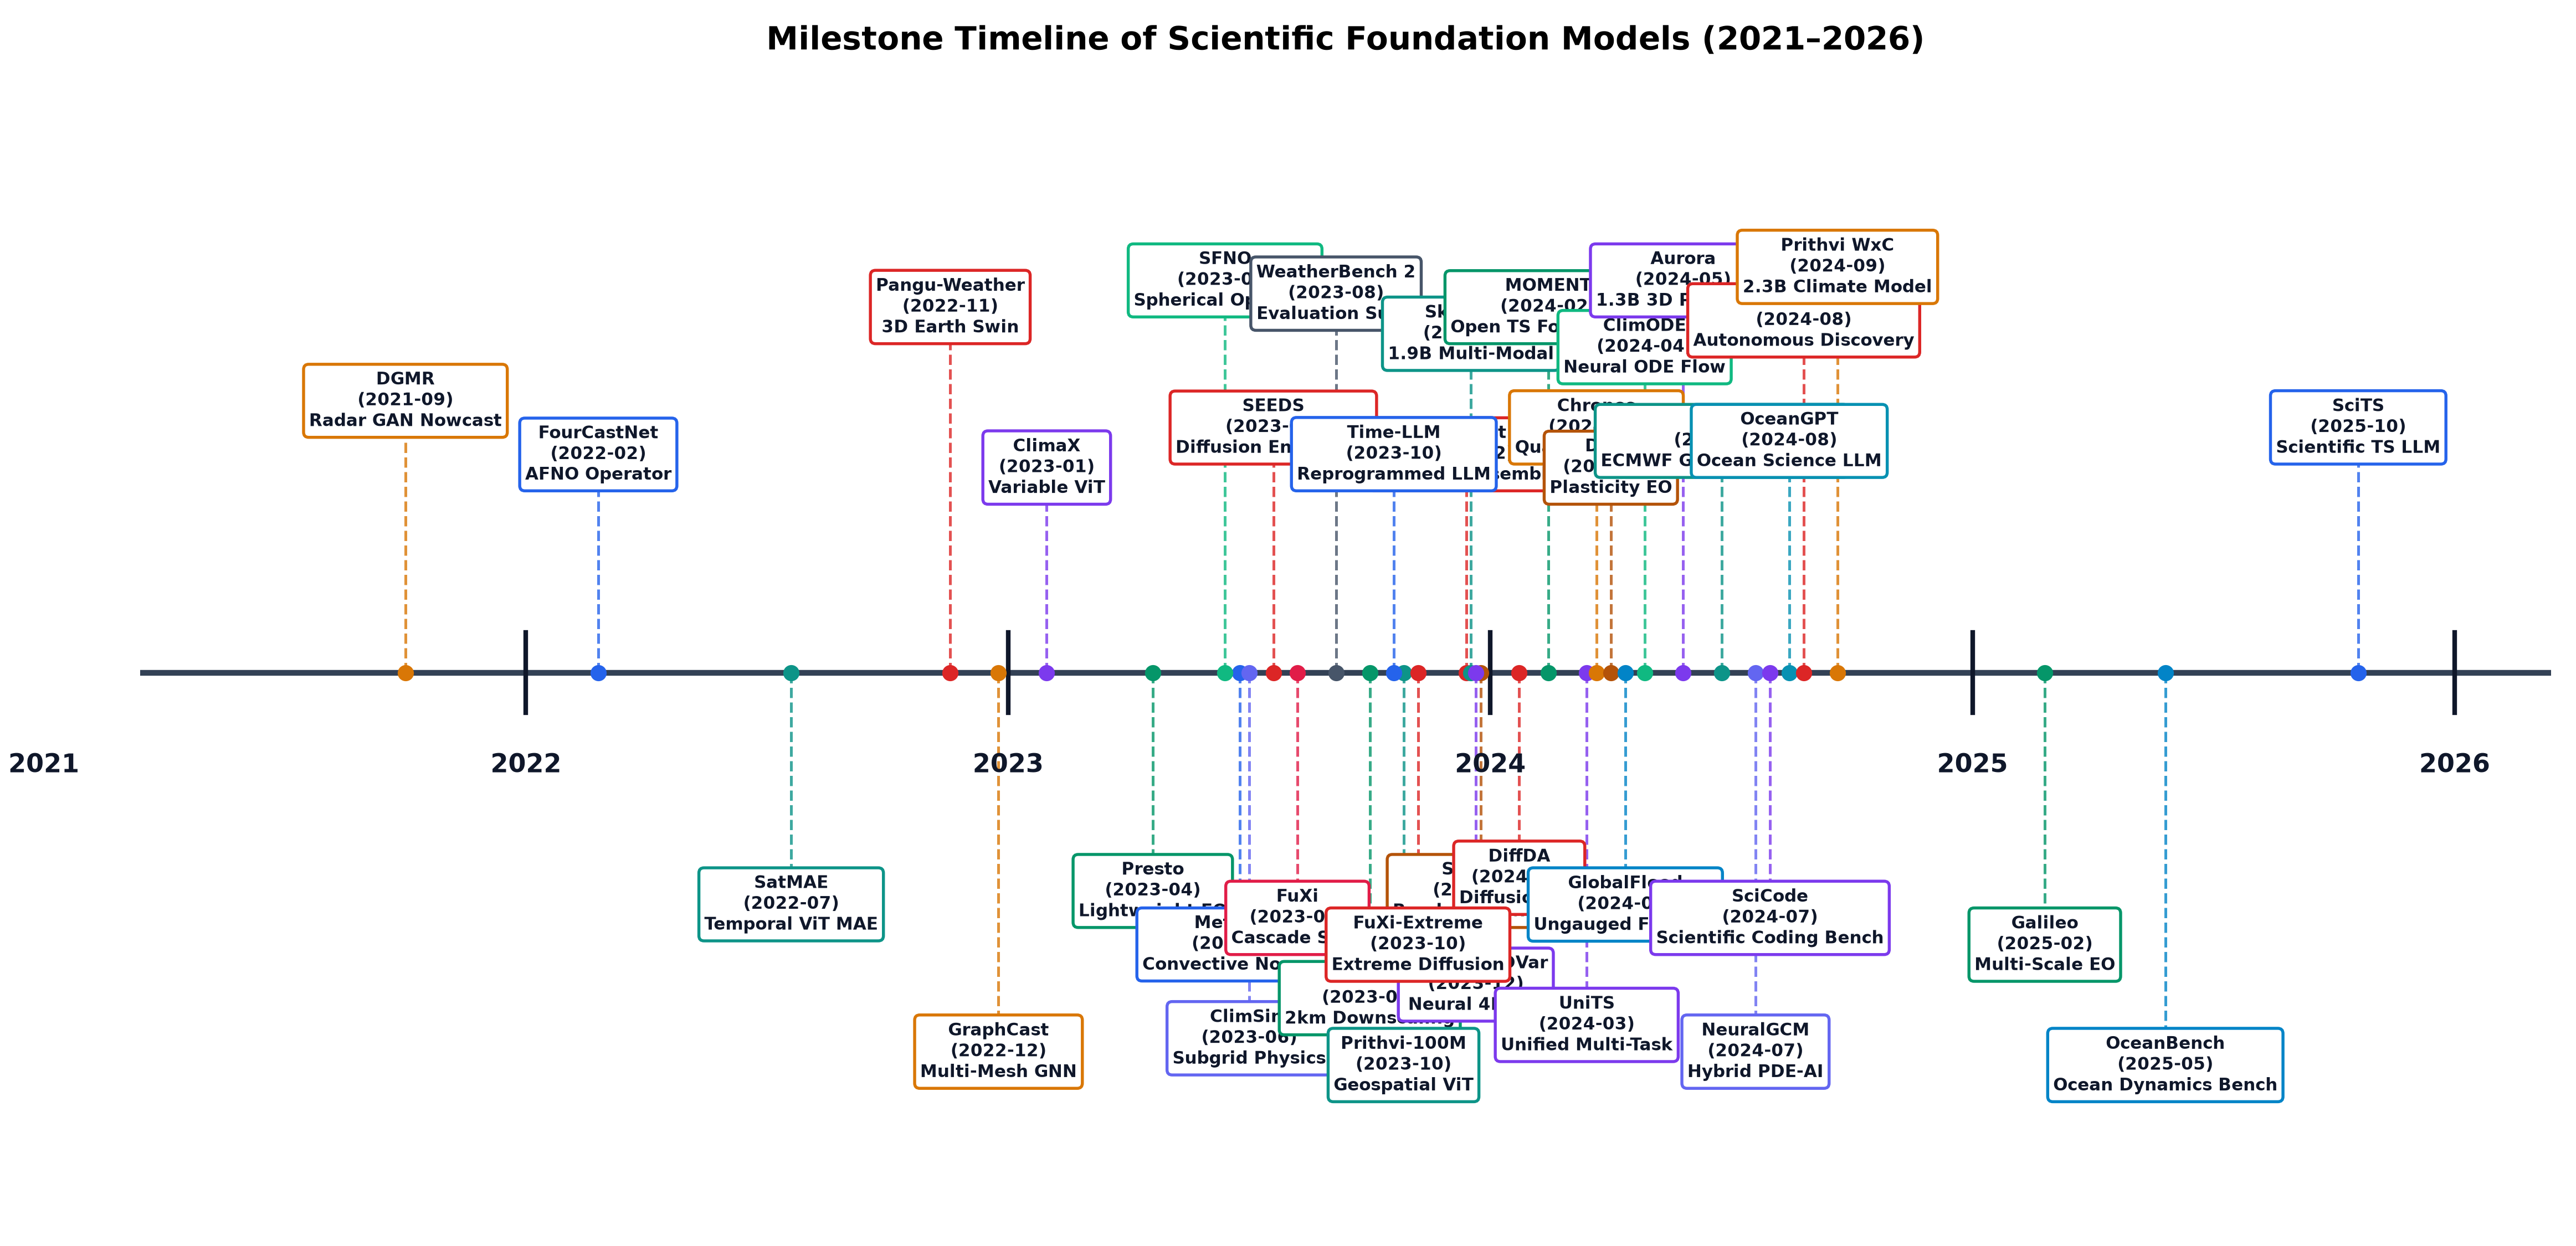
\includegraphics[width=\textwidth]{figures/weather_foundation_timeline.png}
\caption{Milestone timeline of representative scientific multimodal time series foundation models and evaluation frameworks from 2022 to 2026.}
\label{fig:weather_timeline}
\end{figure*}

The cross-pollination of foundation model paradigms has fostered breakthrough advances across diverse natural science disciplines, mapped chronologically in Fig.~\ref{fig:weather_timeline}.

\subsection{Weather and Climate Forecasting}
Global numerical weather prediction represents the flagship proving ground for scientific foundation models. As demonstrated by Pangu-Weather~\cite{bi2023pangu}, GraphCast~\cite{lam2023graphcast}, FuXi~\cite{chen2023fuxi}, FengWu~\cite{chen2023fengwu}, and Aurora~\cite{bodnar2024aurora}, deep learning architectures execute 10-day global forecasts in tens of seconds on a single GPU, delivering computational speedups of $1{,}000\times$ to $10{,}000\times$ compared to operational NWP supercomputing workflows. Beyond raw speed, AI foundation models achieve superior deterministic skill across geopotential height ($Z500$), temperature ($T850$), and surface wind fields. Furthermore, versatile foundation models such as ClimaX~\cite{nguyen2023climax} demonstrate multi-task transferability by pretraining on synthetic CMIP6 climate projections and fine-tuning for regional climate downscaling and seasonal teleconnections.

\begin{figure}[t]
\centering
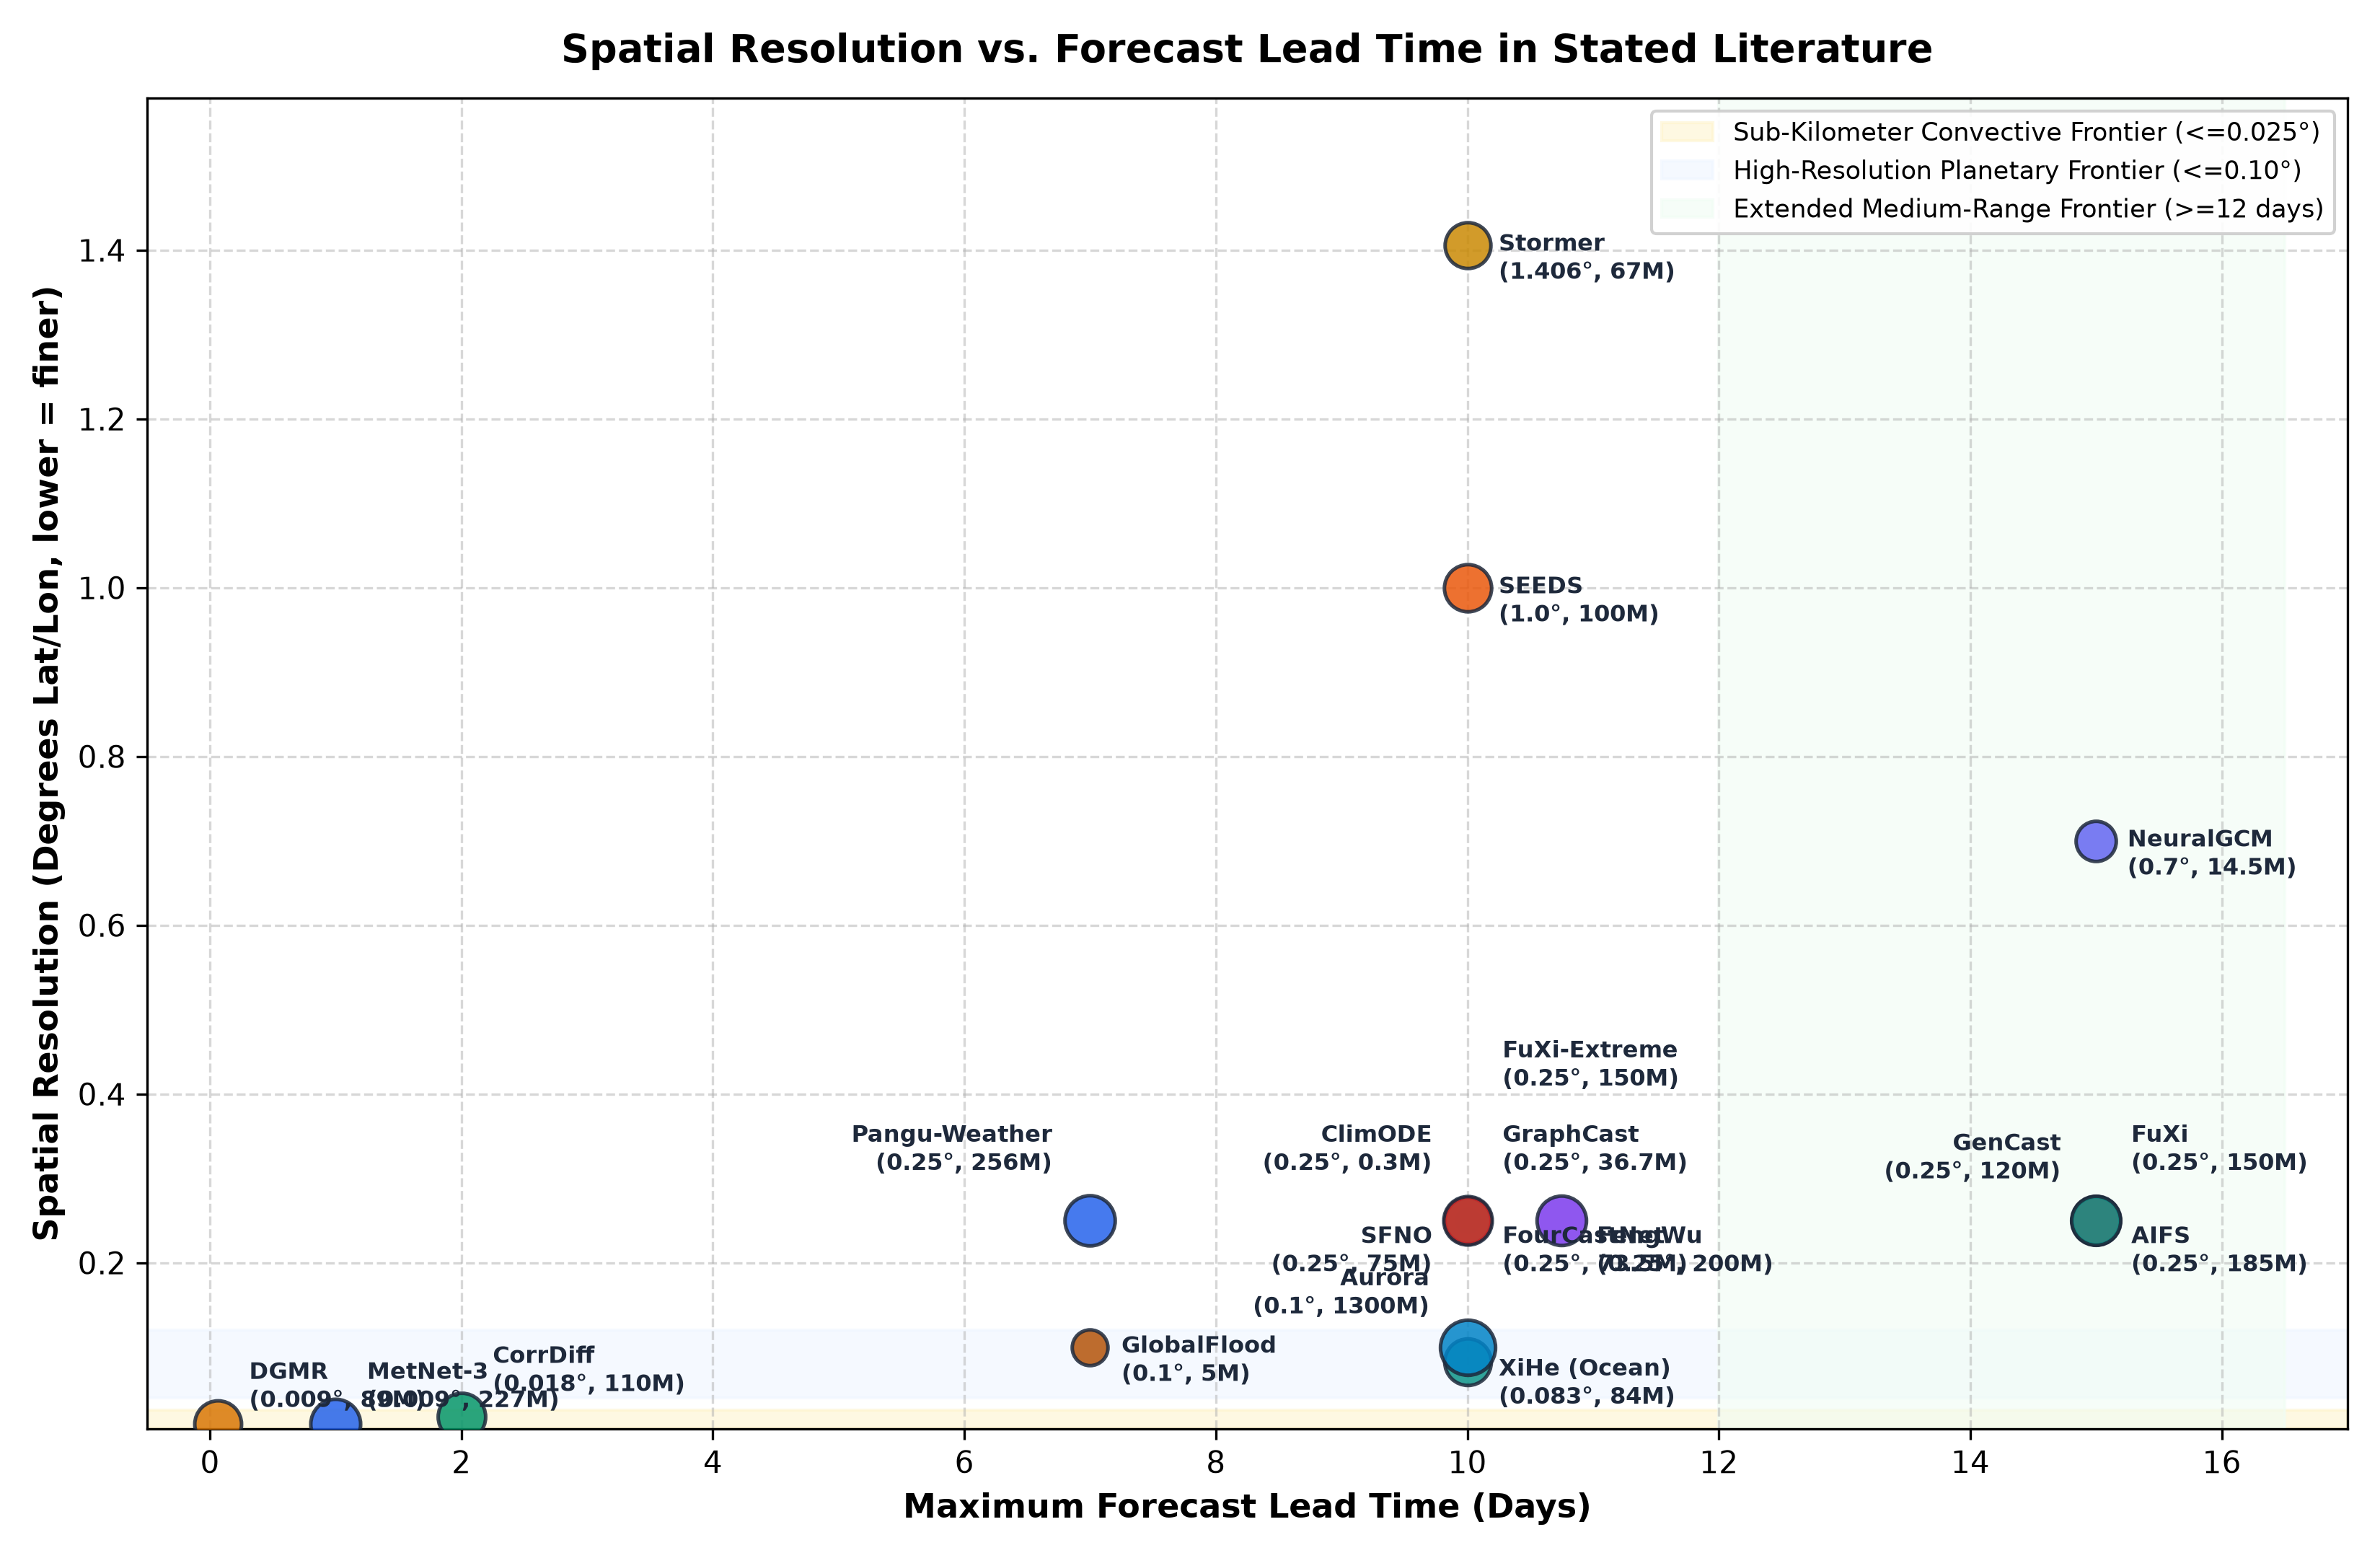
\includegraphics[width=\columnwidth]{figures/resolution_vs_leadtime.png}
\caption{Spatial resolution (degrees latitude/longitude) versus maximum forecast lead time (days) for verified scientific foundation models. Marker size is proportional to log model parameter count.}
\label{fig:res_vs_leadtime}
\end{figure}

As shown in Fig.~\ref{fig:res_vs_leadtime}, current state-of-the-art models occupy distinct Pareto trade-offs: while deterministic models like Pangu-Weather and GraphCast optimize accuracy at standard $0.25^\circ$ resolution across 7--10 days, frontier models like Aurora advance spatial resolution to $0.1^\circ$, and cascade systems (FuXi) or diffusion ensembles (GenCast) extend skillful forecasting horizons out to 15 days.

\subsection{Sub-Kilometer Convective-Scale Emulation and Generative Downscaling}
\label{sec:convective_downscaling}
A fundamental limitation of global foundation models (operating at $0.25^\circ \approx 25\text{--}31\text{ km}$ or $0.1^\circ \approx 10\text{ km}$) is their inability to resolve sub-kilometer convective phenomena. Convective thunderstorms, microbursts, urban flash flooding, and complex orographic wind channeling occur at localized scales ($< 3\text{ km}$) where non-hydrostatic atmospheric dynamics dominate. Bridging this multiscale gap has motivated frontier research into generative radar nowcasting and residual diffusion downscaling:
\begin{enumerate}
    \item \textbf{Generative Radar Precipitation Nowcasting: DGMR}: Ravuri et al.~\cite{ravuri2021dgmr} established the landmark \textbf{DGMR} (Deep Generative Model of Radar), deploying spatial-temporal generative adversarial networks for precipitation nowcasting at 1 km spatial and 5-minute temporal resolution across the United Kingdom. Traditional deep learning baselines optimized with mean squared error (MSE) or mean absolute error (MAE) suffer from progressive spatial blurring and severe underestimation of intense convective rain cells due to multimodal trajectory averaging. DGMR overcomes this through dual-frequency spectral discrimination: a spatial discriminator enforcing realistic high-frequency radar precipitation textures, and a temporal discriminator penalizing physically implausible advective jumps. In rigorous double-blind evaluations conducted with professional operational forecasters at the UK Met Office, DGMR was ranked first in 89\% of cases for overall value, physical plausibility, and localized heavy rain cell fidelity compared to optical flow (PySTEPS) and convolutional recurrent baselines.
    \item \textbf{Continental Multi-Sensor Convective Forecasting: MetNet-3}: Andrychowicz et al.~\cite{andrychowicz2023metnet3} scaled convective forecasting across the entire continental United States (CONUS) out to 24-hour lead times at 1--4 km spatial resolution. Operating over a continuous spatial grid ($4{,}096 \times 4{,}096\text{ km}$), \textbf{MetNet-3} assimilates heterogeneous and asynchronous observational modalities directly: high-resolution ground radar composites (MRMS), geostationary satellite multi-spectral imagery (GOES-16), surface meteorological station networks, and numerical forecast initializations (HRRR). Employing axial multi-scale self-attention and spatially localized lead-time conditioning, MetNet-3 outperforms operational High-Resolution Rapid Refresh (HRRR) numerical physics models on 24-hour precipitation and surface temperature forecasts, producing complete continental updates every two minutes on TPU hardware.
    \item \textbf{Kilometer-Scale Residual Generative Downscaling: CorrDiff}: Bridging coarse global foundation model outputs ($25\text{ km}$ ERA5) to local convective scales ($2\text{ km}$), Mardani et al.~\cite{mardani2023corrdiff} formulated \textbf{CorrDiff}, a residual corrective diffusion framework developed for extreme weather prediction over complex topography (Taiwan). Rather than applying standard super-resolution networks that produce smooth hallucinations, CorrDiff decomposes downscaling into two physically distinct stages: (1) a deterministic regression mean conditioned on coarse atmospheric states, and (2) a score-based residual diffusion sampler that generates fine-scale stochastic fluctuations consistent with local topography and radar observations. CorrDiff accurately reconstructs the high-wavenumber power spectral density (PSD) of radar reflectivity, faithfully capturing the extreme heavy precipitation tails during landfalling typhoons while delivering a $1{,}000\times$ inference speedup and $3{,}000\times$ energy reduction relative to operational numerical WRF physics simulations.
\end{enumerate}

\subsection{Earth Observation and Remote Sensing Time Series}
Satellite constellations monitor terrestrial ecosystems, vegetation phenology, and surface hydrological states through high-dimensional spatio-temporal revisit series. Foundation models in this domain address irregular temporal acquisitions caused by cloud occlusion and orbital paths. Models like SatMAE~\cite{cong2022satmae}, Presto~\cite{tseng2023presto}, and Galileo~\cite{tseng2025galileo} leverage self-supervised temporal-spectral masked autoencoding, allowing sparse downstream fine-tuning for global crop classification, wildfire burn scar delineation, and surface water mapping with minimal labeled ground truth. AlphaEarth Foundations~\cite{brown2025alphaearth} further compresses multi-sensor imagery into dense, pixel-level 64-dimensional embedding fields accessible directly through planetary cloud platforms like Google Earth Engine. Scaling foundation models to multi-modal satellite constellations, SkySense~\cite{guo2024skysense} unifies optical and synthetic aperture radar (SAR) time series with 1.9 billion parameters, delivering state-of-the-art transfer performance across land-use mapping, infrastructure monitoring, and temporal change detection benchmarks such as GEO-Bench~\cite{lacoste2023geobench}.

\subsection{Hydrology and Extreme Flood Modeling}
Hydrological forecasting requires predicting water discharge through river networks subject to precipitation forcing, evapotranspiration, and soil infiltration. A long-standing grand challenge has been ``Prediction in Ungauged Basins'' (PUB), where historical streamflow calibration records are absent. Nearing et al.~\cite{nearing2024globalflood} demonstrated that deep learning models trained on 5,680 diverse river basins across the globe achieve unprecedented zero-shot flood forecasting skill in ungauged catchments, extending actionable early warning lead times from 0 to 5 days globally and outperforming the Copernicus GloFAS operational physics-based system. Complementing these architectural advances, Kratzert et al.~\cite{kratzert2023caravan} released Caravan, a standardized global community dataset spanning 6,830 catchments worldwide with unified ERA5-Land meteorological forcings, catchment attributes, and daily streamflow records. By eliminating the geographic fragmentation of regional datasets (e.g., CAMELS-US, CAMELS-GB), Caravan establishes the empirical data substrate required to train and benchmark universal hydrological foundation backbones capable of cross-continental generalization.

\subsection{Oceanography and Marine Systems}
Ocean dynamics govern planetary heat distribution, carbon uptake, and marine biogeochemical cycles. Wang et al.~\cite{wang2024xihe} developed XiHe, a hierarchical ocean transformer trained on 28 years of GLORYS12V1 reanalysis at eddy-resolving $1/12^\circ$ resolution. By incorporating land-ocean boundary masking and multi-level vertical attention, XiHe models mesoscale eddies, sea surface temperature anomalies, and 3D velocity vectors, outperforming traditional operational hydrodynamic models (e.g., PSY4, GIOPS) while generating 10-day global forecasts in under 0.4 seconds. Addressing the extreme sparsity of oceanic observation networks, 4DVarNet~\cite{fablet2021learning} formulates neural variational data assimilation to invert along-track satellite altimetry into continuous 2D sea surface height (SSH) dynamics, demonstrating that learnable unrolled variational solvers reconstruct fine-scale mesoscale eddies and oceanic kinetic energy spectra far more effectively than classical optimal interpolation (OI).

To standardize evaluation across emerging marine foundation models, El Aouni et al.~\cite{elaouni2025oceanbench} established \textbf{OceanBench}, an open operational benchmarking suite for data-driven global ocean forecasting systems developed in collaboration with Mercator Ocean International. OceanBench benchmarks predictive skill for sea surface height (SSH), sea surface temperature (SST), and horizontal current velocities across 1- to 10-day lead times against CMEMS GLORYS12 reanalyses and in-situ altimetry observations. Bridging physical ocean simulations with cross-modal scientific reasoning, Bi et al.~\cite{bi2024oceangpt} introduced OceanGPT, the first domain-specific foundation language model for marine science. Pretrained and aligned on the DoInstruct corpus comprising multimodal oceanographic time series (temperature-salinity profiles from Argo float arrays and mooring buoys), sensor trajectories, and marine scientific literature, OceanGPT demonstrates autonomous reasoning across ocean dynamics, thermohaline circulation changes, and marine phenomenon attribution under physical consistency constraints.

\subsection{Geophysics and Seismology}
In seismology, continuous 3-component acoustic waveforms record tectonic stress accumulation and seismic rupture. While classical phase-picking baselines like PhaseNet~\cite{zhu2019phasenet} utilized supervised 1D U-Nets for local seismic windows, modern foundational architectures such as SeisT~\cite{li2024seist} train hierarchical seismogram transformers on tens of millions of global waveforms. SeisT supports multi-task downstream adaptation, simultaneously performing earthquake detection, high-precision P/S phase picking, initial-motion polarity determination, and magnitude/epicenter regression. Providing the standardized foundational infrastructure for seismic machine learning, Woollam et al.~\cite{woollam2022seisbench} released \textbf{SeisBench}, unifying 30+ million waveforms across global catalogues (ETHZ, GEOFON, INSTANCE, SCEDC, STEAD) into a standardized multi-task evaluation and transfer benchmark.

\subsection{Space Weather and Heliophysics}
Space weather phenomena---including solar flares, coronal mass ejections (CMEs), and geomagnetic storms---exert severe risks on satellite infrastructure and terrestrial power grids. Roy et al.~\cite{roy2025surya} introduced Surya, a 366-million parameter foundation model for heliophysics trained on 13 years of continuous multi-wavelength extreme ultraviolet imagery from NASA's Solar Dynamics Observatory (SDO). Surya incorporates spectral gating and long-short attention to track active region magnetic helicity, delivering state-of-the-art solar flare and solar wind forecasting.

\subsection{Cross-Disciplinary Universal Time Series Foundations}
Bridging physical boundaries between disparate earth science subdomains, universal foundation models like UniTS~\cite{gao2024units} and MOMENT~\cite{goswami2024moment} demonstrate that pretraining on multi-domain scientific collections enables cross-physics zero-shot transfer. By decoupling sequence tokens from variable identities and applying prompt-conditioned task masks, universal backbones can be deployed across river streamflow, power grids, seismic sensors, and atmospheric stations without re-training architectural weights.
